\section{Introduction}
Visual environments can vary significantly depending on the geographical location. Even within the same location certain visual features such as colours, texture, vegetation, prey and predators can change drastically between generations, altering the statistics of the visual scene. Thus, genetically similar individuals of the same species occupy many different ecological niches, presenting unique challenges for the visual system (\cite{Engeszer2007ZebrafishField}). As a result, developing animals must learn the statistics of these environments in order to ensure that the ontogeny of visual behavior can either cope with, or exploit a given ecological niche (\cite{Wong2015BehavioralEnvironments}; \cite{Harer2019RevertingFish}; \cite{Gilmour2018PlasticityConditions}).

Flexibility in the face of such environmental diversity is thought to be achieved through mechanisms of experience-dependent plasticity, where incoming sensory input plays an instructive role in the structural and functional formation of neural circuits (\cite{Fox2005ReviewSystems}; \cite{Hooks2007CriticalPlasticity.}). Whilst experience-dependent plasticity is widespread across different species it has been extensively studied in the retinotectal system of anamiotes (namely fish and frogs) (\cite{Ruthazer2010LearningFunction}; \cite{Pratt2016AnDevelopment}). This is because, unlike their amniotic counterparts (chicks, reptiles and mammals) that develop in the absence of visual input, the development of anamiotes is extremely rapid and entirely external. As a result they rely on complex stimulation from the visual world to pattern the early visual system rather than spontaneously induced waves driven from the retina (\cite{Pratt2016AnDevelopment}).
This allows for activity in the tectum to be altered through manipulations to the visual scene over a time period when visually guided behaviour is first emerging (\cite{Ruthazer2004InsightsPerspective}). Furthermore, due to the accessibility and experimental tractability of the tectum, the effect of these manipulations of retinotectal neurons can be readily observed.

During early tectal development coarse retinotopic maps are first established by \gls{rgc} axons following molecular gradients (\cite{Higenell2012ExpressionLaevis}; \cite{Liu2004SwitchingDevelopment}; \cite{Kita2015TopographicZebrafish}). This map is then refined to mature levels of precision by visual experience (\cite{Ruthazer2004InsightsPerspective}). This topographic refinement is driven through dynamic rearrangement of axon branches, selectively stabilising branches in tectal regions that show correlated activity with the developing axon while eliminating those that do not (\cite{Ruthazer2003ControlVivo}; \cite{Munz2014RapidStimulation}; \cite{Ruthazer2004InsightsPerspective}). RGCs also have been shown to modulate the growth of their target neuron's dendrites (\cite{Sin2002DendriteGTPases}), receptive field properties (\cite{Tao2005Activity-dependentFields}; \cite{Dong2012AFields}; \cite{Engert2002MovingNeurons}) and shape local recurrent circuitry through intra-tectal connections (\cite{Pratt2008DevelopmentTectum}; \cite{Xu2011VisualSystem}). 

Many activity dependent effects are thought to be driven by mechanisms of Hebbian plasticty through STDP where the relative timing between pre- and postsynaptic spikes can either strengthen synapses through LTP or weaken them through LTD (\cite{Mu2006SpikeSystem}; \cite{Zhang1998ASynapses}; \cite{Richards2010InLaevis}). Such mechanisms are thought to be mediated by the NMDAR, which acts as a molecular detector of correlated activity. Consistent  with this, many experience-dependent effects can be abolished through selective blockade of the \gls{nmda}  (\cite{Ruthazer2003ControlVivo}; \cite{Engert2002MovingNeurons}; \cite{Sin2002DendriteGTPases}; \cite{Kutsarova2017RulesBrain}). However, Hebbian mechanisms are not the only way that experience shapes the developing visual system. For example, enhanced visual input causes homeostatic changes in the intrinsic excitability of tectal neurons, adjusting their gain to improve stimulus detection (\cite{Aizenman2003VisuallyVivo}; \cite{Pratt2007HomeostaticCircuit}). In contrast, the overall number of cells in the tectum, can be decreased by lowering ambient light levels, suggesting that the neurogensis rate is also regulated by sensory input (\cite{Hall2018VisualTectum}). Together these studies suggest that visual experience has wide spread effects on the development of the tectum.

Recently, a number of studies have taken advantage of the small size and optical clarity of the anamiotic optic tectum to assess the impact of visual experience on developing population activity by using calcium imaging techniques. This is an important development because behaviour and sensory representations are likely to be encoded through the coordinated activity of groups of neurons organised into neural assemblies, rather than single neurons (\cite{Yuste2015}). In tadpoles, visually evoked correlated activity in the tectum increases over the course of development, a process that is abolished through dark rearing or \gls{nmda} blockade (\cite{Xu2011VisualSystem}). In zebrafish, looking at the development of spontaneous activity, it was found that neural assembly number, size and correlation initially increased (2.5-5 \gls{dpf}) and then decreased (5-7 \gls{dpf}) (\cite{Avitan2017}). These tectal neural assemblies were still present in the absence of visual stimulation and, despite removal of the eye, remained predictive of tail movements (\cite{Avitan2017}; \cite{Pietri2017}). This suggests that the development of neural assemblies may rely on principally on intrinsic factors (\cite{Pietri2017}). However, dark rearing caused neural assemblies to be fewer in number, less correlated and severely impacted the ability of the fish to hunt prey (\cite{Avitan2017}). These results indicate that while both intrinsic and extrinsic factors are important for shaping tectal population activity, visual input is necessary for the emergence of hunting behaviour.

In the wild, zebrafish have been found to thrive in different environments scattered across southern Asia and these environments display extreme diversity in terms of the visual features they contain (\cite{Engeszer2007ZebrafishField}).  However, the manipulations that are often used to study how experience shapes the brain in the lab such as dark rearing, monocular deprivation and 
sustained presentations of artificial stimuli are devoid from any naturalistic change that zebrafish would usually experience. Even in the absence of such manipulations normal rearing conditions for model organisms within the lab are highly impoverished, possibly perturbing natural visual system development. An alternative strategy is to use \gls{ee}, rearing conditions that are designed to increase cognitive, motor or sensory stimulation in regards to typical laboratory rearing conditions. In mice, housing with natural bedding,  novel objects and exercises wheels has shown to have wide ranging effects on behaviour, cognitive ability, anxiety and visual system development (\cite{Nithianantharajah2006EnrichedSystem, Beaulieu1990EffectProperties,Beaulieu1987EffectCortex, Mainardi2010EnvironmentalCortex,Sale2007EnvironmentalInhibition}). However, all of these studies enrich multiple different sensory modalities. Currently no study has looked exclusively at the effect of visual enrichment on the developing nervous system and particularly its effect on the emergence of visually guided behaviour and population activity.

In this chapter I sought to understand how natural vision impacts behaviour and development of population activity. larval zebrafish were raised either within normal laboratory rearing conditions (on a shelf in the incubator) or within an enriched visual environment. This \gls{EE} consisted of placing gravel under the petri dish contianing the developing larvae. To examine the effect of enrichment on behaviour \gls{nr} and \gls{gr} fish were allowed to hunt prey within either a \gls{gb} or \gls{wb}. This revealed that GR fish consumed more prey exclusively when hunting over the \gls{gb}, indicating that they may have learnt to use features of the environment to increase their hunting performance. Using 2-photon volumetric imaging to capture the activity of thousands of neurons throughout the optic tectum combined with Bayesian inference techniques showed that \gls{ee} has a profound effect on neural assembly development, with assembly size, firing frequency and synchrony all showing divergent developmental trajectories between 5 and 7 \gls{dpf}. These results suggest that \gls{ee} modifies the structure of population activity in the tectum and that this correlates with improved performance of a tectally-mediated hunting behaviour in a complex visual environment.  Finally, to understand which forms of plasticity may be underlying these experience-dependent changes we generated zebrafish carrying null mutations in \textit{grin2aa} and \textit{grin2ab} which code for isoforms of the NR2A subunit of the \gls{nmda} receptor. In these fish that the effects of \gls{ee} were found to be  blocked, suggesting that the subunit composition of the \gls{nmda} is crucial for mediating the effects of \gls{ee} on functional development of the tectum.
 
\section{Results}
Under laboratory conditions embryonic zebrafish usually develop in a petri dish placed on a shelf within an incubator. These rearing conditions bear little resemblance to the zebrafish's natural habitat lacking many natural features of the visual scene (\cite{Engeszer2007ZebrafishField}). In order to understand how changes in the visual environment affect the development of visually guided behaviour and population activity, zebrafish were either raised under typical lab conditions or in a petri dish rested on a bed of gravel (gravel was also piled around the side of the dish) from 1-7 \gls{dpf}. Both conditions were fed rotifers (live prey) daily from the evening of 4 \gls{dpf} onwards (\textbf{Figure \ref{fig:R2_F1}}).  Placing gravel under the dish exclusively enriches the visual environment by providing natural features that are lacking from the NR condition such as color, texture and diverse spatial frequencies. Furthermore unlike previously used \gls{ee}s, this is purely a visual manipulation with the fish being physically separated from the gravel, therefore the gravel does not provide any potential tactile, olfactory or gustatory stimulation.

\begin{figure}[!ht]
        \center{\includegraphics[width =  0.5\paperwidth]{Figures/R2_F1.pdf}}
            \caption[\textbf{\label{fig:R2_F1}Enriching the visual environment.}]{ \textbf{\label{fig:R2_F1} Enriching the visual environment.} To alter the visual environment zebrafish were either raised over a bed of gravel (GR) or under normal laboratory conditions, with the dish placed on a shelf within the incubator (NR). The NR condition lacks many of the features of the natural world with the fish seeing only the white colour of the incubator and the metal grating of the shelf below their dish.  Adding gravel adds a number of natural features that are absent from the NR condition, such as different colours, curved edges, contrast, different spatial frequencies and stronger optic flow as the fish swims. Therefore GR creates an \gls{ee} when compeared to the NR condition.}
      \end{figure}
      



\subsection{Enrichment enhances prey consumption in a complex visual scene}
To understand the effect of the \gls{ee} on the emergence of visually guided behaviour NR and GR were put through a hunting assay. Based on the different rearing conditions it is possible that any effect on behaviour would be specific to that is specific to the environment. To test this NR and GR fish from the same clutch were added to 35 mm petri dishes containing rotifers and then were placed to hunt for 30 mins over either a \gls{wb} or a \gls{gb}. These dishes were imaged for $\sim$30 seconds prior to and after hunting to record the number of rotifers in the dish (\textbf{Figure \ref{fig:R2_F2} A-C}). The number of rotifers then were manually counted to give before and after readings. This allowed for the number of rotifers consumed in each hunting session to be estimated. Prior to counting the rearing condition was blinded to the counter in order to remove bias.

\clearpage
\begin{figure}[]
        \center{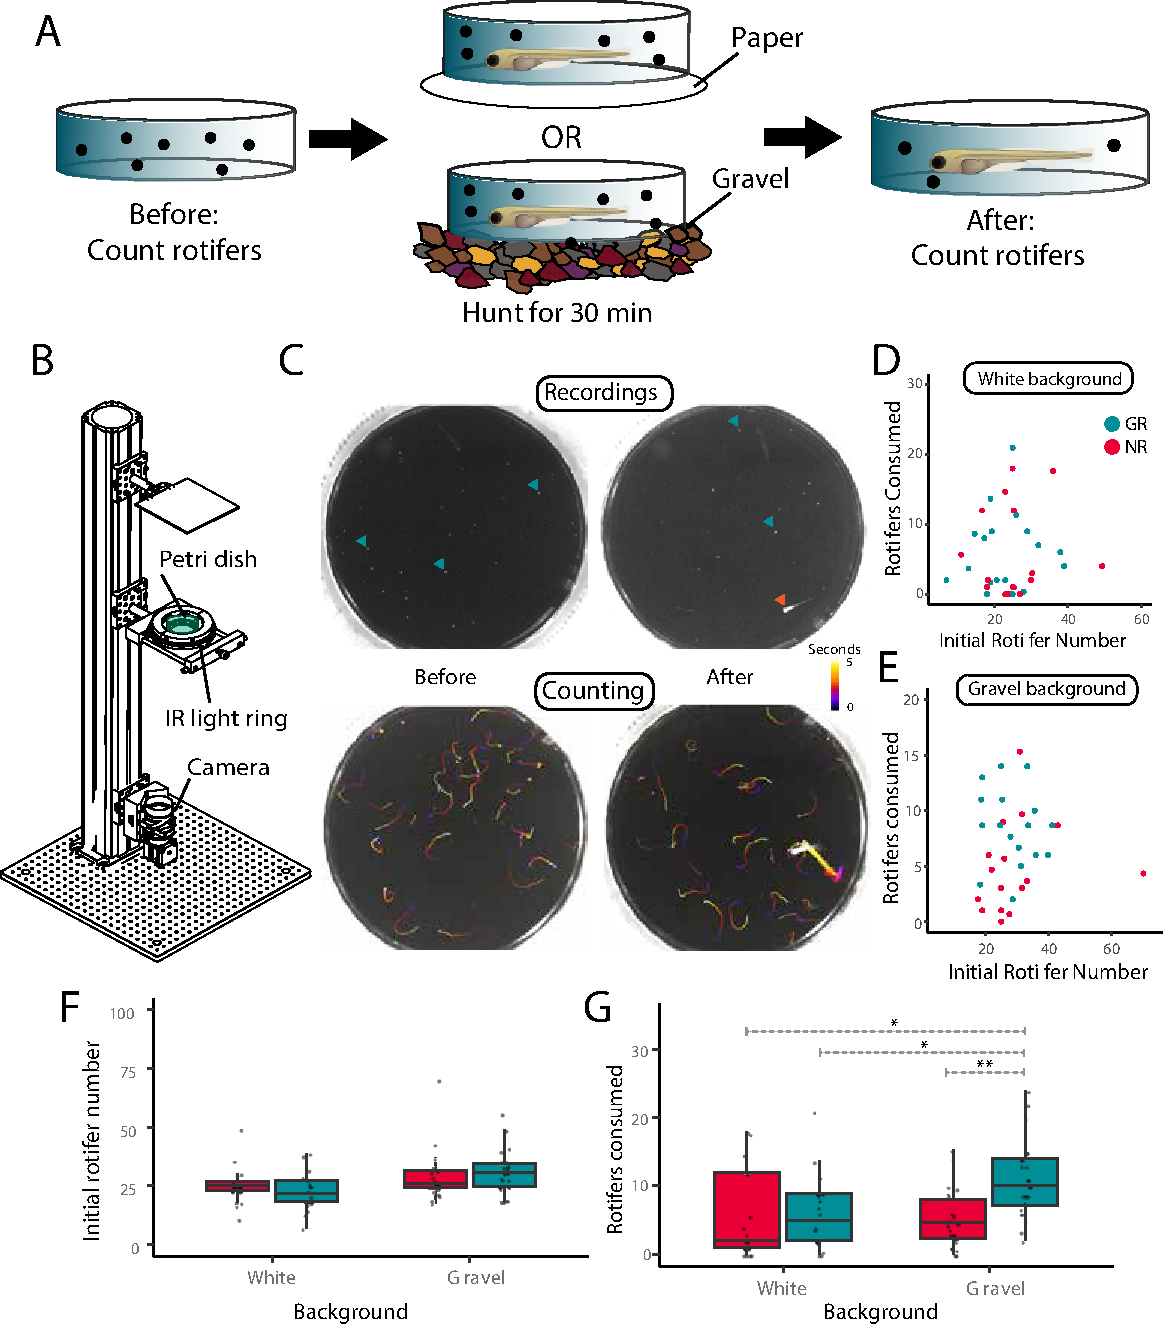
\includegraphics[width =  0.7\paperwidth]{Figures/R2_F2_v3.pdf}}
            \caption[\label{fig:R2_F2} \textbf{The effect of EE on hunting behaviour}]{\label{fig:R2_F2} \textbf{The effect of EE on hunting behaviour} \textbf{(A)} GR and NR fish were subjected to a hunting assay where rotifers were added to a petri dish placed over a white sheet of paper or a bed of gravel. The initial number of rotifers in the dish was counted and fish were then left to hunt for 30 mins. After this period, the number of rotifers was re-counted to estimate the number of rotifers consumed.\textbf{(B)} Behavioural set up for imaging rotifers. The petri dish containing the rotifers was placed in the center of a ring containing infrared LEDs and then imaged by a camera sitting below \textbf{(C) Top:} Example frames from the raw recordings of rotifers before and after hunting (Green arrows point to rotifers; Red arrow points to a zebrafish larvae).\textbf{Bottom:} By colouring frames of the movie by time the swimming trajectories of rotifers could be visualised making them easier to manually count. \textbf{(D-E)} Scatter plots showing the relationship between the initial number of rotifers and the rotifers consumed in 30 mins (\gls{wb}: r = 0.06, p = 0.7, \gls{gb}: r = 0.2, p = 0.09). \textbf{(F)} The initial number of rotifers in the dish prior to hunting was similar across all conditions (WB NR vs WB GR: p = 1, GB NR vs GB GR:  p = 1, WB NR vs GB NR: p = 1, WB GR vs GB GR: p = 0.07,  WB GR vs GB NR:  p = 0.29, WB NR vs GB GR: p = 0.21, Mann Whitney U tests)\textbf{(G)} Box plot showing the number of rotifers consumed within 30 mins when over the white background and gravel background (WB NR vs WB GR: p = 1, GB NR vs GB GR:  p = 0.003, WB NR vs GB NR: p = 1, WB GR vs GB GR: p = 0.026,  WB GR vs GB NR:  p = 1, WB NR vs GB GR: p = 0.26, Mann Whitney U tests). All multiple comparisons were corrected using the Bonfferoni method. \text{*} : p < 0.05; \text{**} : p < 0.01; \text{***}: p < 0.001. box plots represent median and interquartile range.}
      \end{figure}

It may be expected that the density of rotifers could affect the hunting performance of zebrafish. To examine if the number of rotifers affected hunting performance, the initial number of rotifers in the dish was plotted against the number of rotifers consumed for both white and gravel backgrounds.  This showed that there was no relationship between rotifer density and hunting performance (\gls{wb}: r = 0.06, p = 0.7, \gls{gb}: r = 0.2, p = 0.09) (\textbf{Figure \ref{fig:R2_F2} D-E}). Furthermore, the was no significant difference in the initial number of rotfiers for any of the conditions (\textbf{Figure \ref{fig:R2_F2} F}). This indicates that the rotifer density is unlikely to be a confounding factor when looking at the effect of EE on prey consumption. This allowed for the effect of \gls{ee} on prey consumption to be assessed by looking at the total number of rotifers consumed within each of the hunting assays. It revealed that when hunting over the white background GR and NR fish consumed a similar number of rotifers (WB NR vs GR: p = 1) and when hunting over the GB NR fish showed no difference in their food consumption compared to a WB (WB NR vs GB NR: p = 1, WB GR vs GB NR: p = 1). GR fish on the other hand showed a specific increase in the number of prey they were consuming when hunting over the gravel background compeared to all other conditions (GB NR vs GB GR: p = 0.003, WB NR vs GB GR: p =  0.026, WB GR vs GB GR: p =0.026, Mann-Whitney U test, Bonferroni correction)  (\textbf{Figure \ref{fig:R2_F2} G}). These results suggest that EE enhances hunting specifically within the complex visual environment of the \gls{gb}.


\subsection{Spontaneous firing properties of tectal neurons are changed by enrichment}
 In zebrafish, the optic tectum contains the neural circuitry that is responsible for directing prey capture (\cite{Gahtan2005}; \cite{Bianco2015}). As the hunting performance is modified by visual experience it is likely that neural circuitry within the tectum is also changing either as a consequence of changes within the retina, within the tectum itself, or both. Therefore to understand how enrichment alters tectal circuitry spontaneous neural activity was recorded from the optic tectum of NR and GR fish at multiple different stages of development (3, 5, and 7 \gls{dpf}) (\textbf{Figure \ref{fig:R2_F3} A}). This allowed for any changes in population activity between rearing conditions to be identified alongside the developmental timepoint at which they occurred. 
 
 Visual experience has previously been shown to homeostaticly alter the intrinsic excitability of cells (\cite{Aizenman2003VisuallyVivo}; \cite{Pratt2007HomeostaticCircuit}) and modify synaptic plasticity (\cite{Mu2006SpikeSystem}), both of which may affect the activity of single neurons within the tectum. Therefore metrics characterising the activity of single tectal neurons were calculated for fish from both groups at each time point. These results were analysed with a two-way \gls{anova} to look at the effects of rearing condition, age and their interaction. Depending on significance these were followed by post-hoc pairwise comparisons on either the main effects, or in the case of significant interaction, on all pairwise comparisons between the factors (rearing condition and age). All multiple comparisons were corrected using the Benjammani-Hochberg method and only the most salient comparisons are reported here for clarity. This analysis revealed that whilst GR and NR fish had similar numbers of active neuron from 3 - 5 \gls{dpf} there were 20.14\% more active cells in GR fish compared to NR fish at 7 \gls{dpf} (NR vs GR 3 \gls{dpf}: p = 0.14, NR vs GR 5 \gls{dpf}: p = 0.099, NR vs GR 7 \gls{dpf}: p = 0.050, two-way ANOVA, interaction:  F(2,33) =6.82, p = 0.003) (\textbf{Figure \ref{fig:R2_F3} B}).  There was no interaction effect for the firing frequency of tectal neurons but independent main effects were seen for rearing condition (F (1,19) =11.38, p = 0.001) and age (F(2,19) 7.26, p = 0.002) independently with a significant increase in firing frequency over the course of development (3 vs 5 \gls{dpf}: p = 0.001, 3 vs 7 \gls{dpf}: p = 0.004) (\textbf{Figure \ref{fig:R2_F3} C}). Likewise main effects but no interaction were also seen for response amplitude (age:  F(2,19) = 5.094, p = 0.011, rearing condition: F(1,19) = 43.08, p < 0.001) and response duration (rearing condition: F(1,19) = 36.70, p < 0.001) with responses being larger and of longer duration in the GR fish (\textbf{Figure \ref{fig:R2_F3} D-E}).  This indicates that \gls{ee} increases tectal neuron activity by increasing the firing frequency, response amplitude and response duration. However, enrichment has a more delayed effect on the number of active neurons which only showed differences in the later stages of development.

\begin{figure}[]
        \center{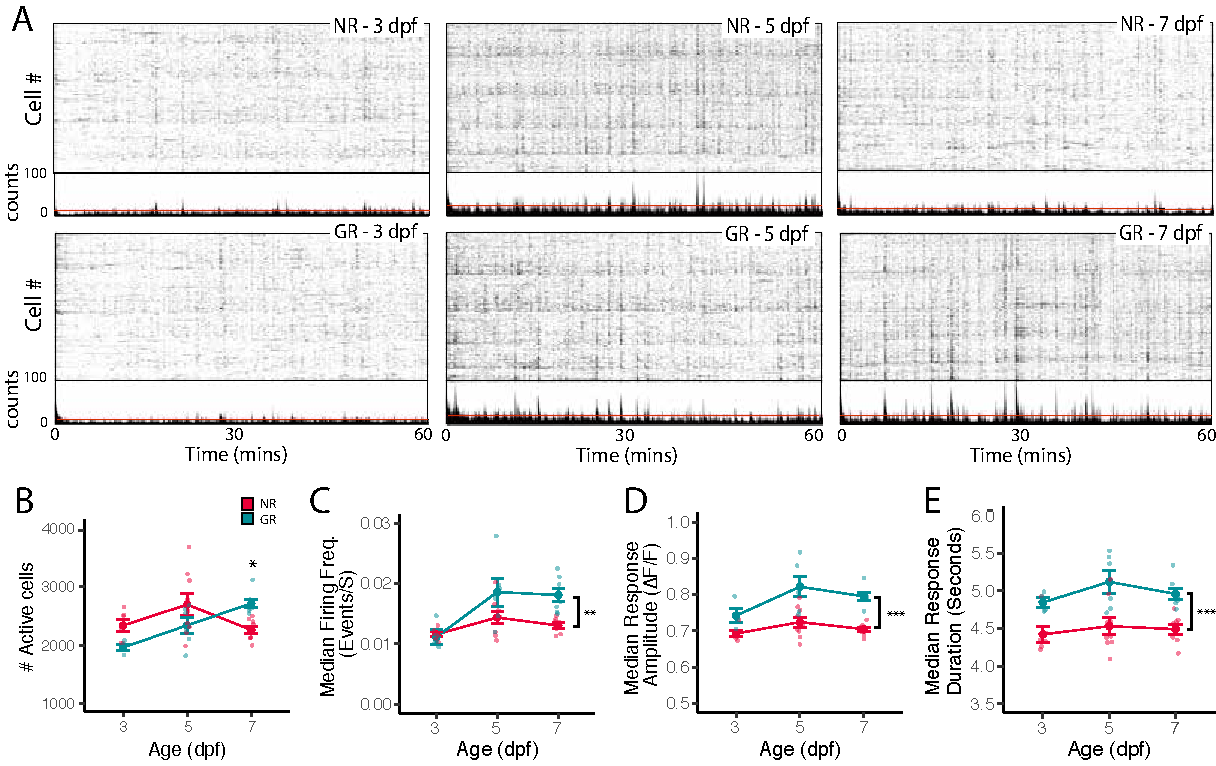
\includegraphics[width =  0.75\paperwidth]{Figures/R2_F3_2.pdf}}
            \caption[\label{fig:R2_F3} \textbf{EE alters the spontaneous properties of single neurons during development.}]{\label{fig:R2_F3} \textbf{EE alters the firing properties of tectal neurons during development. (A)} Representative raster plots of spontaneous activity recorded from the optic tectum of both GR and NR fish at 3, 5, and 7 \gls{dpf}. (NR: 3 \gls{dpf} n = 6, 5 \gls{dpf} n = 9, 7 \gls{dpf} n = 8; GR: 3 \gls{dpf} n = 4, 5 \gls{dpf} = 5, 7 \gls{dpf} = 7). \textbf{(B)} GR fish show an increased number of active cells at 7 \gls{dpf} but not 3 or 5 \gls{dpf} . (GR vs NR: 3 \gls{dpf} p = 0.14, 5 \gls{dpf} p = 0.1, 7 \gls{dpf} p = 0.008; two-way ANOVA, interaction: F(2,33) = 6.82, p =  0.003) \textbf{(C)} Firing frequency was increased in GR fish with respect to NR fish (two-way ANOVA, Age: F(2,19) = 7.6, p = 0.002; Rearing condition: F(1,19) = 11.38, p = 0.002, interaction: f(2,33) =  2.57, p = 0.09). \textbf{(D)} Median response amplitude was increased in GR fish relative to NR fish (two-way ANOVA, Age: F(2,33) = 5.09, p = 0.012; Rearing condition: F(1,33) = 43.07, p < 0.001, interaction: f(2,33) =  1.3, p = 0.29). \textbf{(E)} Median response duration was increased in GR fish compared to NR fish (two-way ANOVA, Age: F(2,33) = 1.69, p = 0.2; Rearing condition: F(1,33) = 36.59, p < 0.001, interaction: f(2,33) =  0.5, p = 0.51). Asterisks highlight contrasts between rearing conditions at each age. All multiple comparisons were corrected using the Benjamani-Hoschberg method. \text{*} : p < 0.05; \text{**} : p < 0.01; \text{***}: p < 0.001. Error bars indicate \gls{sem}.
            }
      \end{figure}



\subsection{Enrichment modifies the developmental trajectory of neural assemblies in the tectum}
Having looked at the effect of \gls{ee} on the development of single neurons properties I next asked whether enrichment alters the structure of population activity in the tectum by analysing the development of tectal assemblies. For this purpose neurons were grouped into assemblies using the BINA clustering method (as described in \textbf{chapter 1}) (\textbf{Figure\ref{fig:R2_F4} A}). 

While the number of assemblies at 5 and 7 dpf was greater than at 3 dpf, rearing conditions had no significant effects on assembly number at any of the three developmental stages (Pooled across rearing condition 3 vs 5 \gls{dpf}: p = 0.023, 3 vs 7 \gls{dpf}: p = 0.030, age: F(2,33) = 4.91, p = 0.01) (\textbf{Figure\ref{fig:R2_F4} B}). The overall percentage of tectal neurons that could be reliably assigned to any of the assemblies  also appeared to increase over development and revealed significant interaction between rearing condition and age (interaction: F (2,33) = 4.45, p = 0.019) with 5 \gls{dpf} GR fish showing a 16\% increase in the number of neurons that could be assigned when compared to NR fish of the same age (5 \gls{dpf} NR vs GR: p = 0.007) (\textbf{Figure\ref{fig:R2_F4} C}). The average number of neurons in each assembly, on the other hand,  followed the same developmental trajectory between GR and NR fish from 3-5 \gls{dpf} but diverged from 5-7 \gls{dpf} resulting in a significant interaction between rearing condition and age (interaction: F(2, 33) =  5.39, p = 0.009) with 7 \gls{dpf} GR fish having 37.4\% more neurons than 7 \gls{dpf} NR fish of the same age (p = 0.0071) (\textbf{Figure\ref{fig:R2_F4} D}). Based on this change it may be expected that the spatial extent of assemblies was also affected. However, there was no interaction between rearing condition and age for the spatial extent of assemblies in the tectum (interaction: F(2, 33) =  0.18, p =  0.85) (\textbf{Figure\ref{fig:R2_F4} E}). In addition, the laterality of the assemblies was also similar between GR and NR fish at all time points, resulting in no interaction (interaction: F(2, 33) =  1.69, p =  0.19). However there was a main effect of age (age: F (2,33) = 5.84, p = 0.007) with assemblies of both rearing conditions combined becoming more lateralised over development (3 vs 5 \gls{dpf}: p = 0.05, 3 vs 7: p = 0.003) (\textbf{Figure\ref{fig:R2_F4} F}). 

 In order to measure the effect of enrichment on assembly dynamics, I plotted assembly frequency, synchrony, and asynchrony against time for each group. Both assembly firing frequency and synchrony in GR fish followed the trajectory of NR fish from 3 - 5 \gls{dpf} but then diverged from 5 - 7 \gls{dpf}. This resulted in the assemblies of 7 \gls{dpf} GR fish being more active (p = 0.044) and less synchronous (p = 0.045) than those of 7 \gls{dpf} NR fish (\textbf{Figure\ref{fig:R2_F4} G-H}). Assembly asynchrony  however remained largely unaffected by rearing condition and age (interaction:  F(2,33) = 2.69, p = 0.083) (\textbf{Figure\ref{fig:R2_F4} I}).

These results demonstrate that the number of assemblies, their spatial extent and laterality are largely unaffected by changing the visual environment with fish from both rearing conditions, showing similar values across development. However, whilst the assemblies of GR and NR fish appear to recruit similar numbers of neurons in early development their developmental trajectories diverge between 5 - 7 \gls{dpf} with the tecta of GR fish possessing much larger assemblies. Furthermore, this divergent change in the developmental trajectory of assemblies is also seen in their dynamics with GR fish showing increased firing frequency and decreased synchrony at 7 \gls{dpf}. These findings suggest that there is a specific developmental time-point, between 5 and 7 \gls{dpf}, during which the visual environment can profoundly alter the developmental trajectory of tectal dynamics.

\begin{figure}[!ht]
        \center{\includegraphics[width =  0.78\paperwidth]{Figures/R2_F4_V2.pdf}}
            \caption[\label{fig:R2_F4} \textbf{The effect of EE on the development on tectal neural assemblies}]{\label{fig:R2_F4} \textbf{The effect of EE on the development on tectal neural assemblies (A)} Raster plots with tectal neurons sorted by their assembly membership for GR and NR fish at 3, 5 and 7 \gls{dpf}. \textbf{(B)} Assembly number increased over the course of development and was unaffected by rearing condition (Age: 3 vs 5 \gls{dpf} p =  0.009, 3 vs 7 \gls{dpf} p = 0.01, 5 vs 7 \gls{dpf} p =  0.64; two way ANOVA, Age: F(2,33) = 4.92, p = 0.013, Rearing condition: F(1,33) = 0.006, p = 0.94, interaction: f(2,33) = 1.81, p = 0.18). \textbf{(C)} The proportion of neural assemblies that can be assigned to an assembly in GR fish is larger at 5 \gls{dpf} than NR fish (GR vs NR: 3 \gls{dpf}  p = 0.28, 5 \gls{dpf} p < 0.001, 7 \gls{dpf} p = 0.28; two way ANOVA, interaction: F(2,33) = 4.45, p = 0.02). \textbf{(D)} The average assembly size, in terms of the number of neurons it recruits, is the same in GR and NR fish at 3 and 5 \gls{dpf} but GR fish have larger assemblies at 7 \gls{dpf} (NR vs GR: 3 \gls{dpf} p = 0.9, 5 \gls{dpf} p = 0.7, 7 \gls{dpf}  p = 0.002; two-way ANOVA, interaction: F(2,33) = 5.4, p = 0.009).  \textbf{(E)} The spatial extent of the assemblies was unaffected by age and rearing condition (two-way ANOVA, Age: F(2,33) = 2.23, p = 0.12, Rearing condition: F(1,33) = 1.39, p = 0.25, interaction: F(2,33) = 0.17, p = 0.85). \textbf{(F)} Assembly laterality was unaffected by rearing condition but increased from 3 \gls{dpf} onwards (3 vs 5 \gls{dpf}: p = 0.04, 3 vs 7 \gls{dpf}: p = 0.003, 5 vs 7 \gls{dpf}: p = 0.81; two way ANOVA, Age: F(2,33) = 5.84, p = 0.007, Rearing condition: F(1,33) = 1.36, p = 0.25, Interaction: F(2,33) = 1.69, p = 0.19). \textbf{(G)} Assembly firing frequency is increased at 7 \gls{dpf} but not at 3 and 5 \gls{dpf} (NR vs GR: 3 \gls{dpf} p = 0.96, 5 \gls{dpf} p = 0.52, 7 \gls{dpf} p =  0.015; two way ANOVA (with white adjustment), interaction = F(2,33) = 3.53, p = 0.04). \textbf{(H)} Assembly synchrony is similar at 3 and 5 \gls{dpf} but is lower in GR fish at 7 \gls{dpf} (NR vs GR: 3 \gls{dpf} p = 0.16, 5 \gls{dpf} p = 0.99, 7 \gls{dpf} p = 0.027, two way ANOVA, Interaction: F(2,33) = 4.67, p = 0.01). \textbf{(I)} Assembly Asynchrony was reduced in GR fish with no effect of age (two way ANOVA, Age: F(2,33) = 1.41, p = 0.26, Rearing condition: F(1,33) = 7.6, p = 0.009, Interaction: f(2,33) = 2.69, p = 0.08). All multiple comparisons were corrected using the Benajamani-Hoschberg method. \text{*} : p < 0.05; \text{**} : p < 0.01; \text{***}: p < 0.001. Error bars indicate SEM.
            }
      \end{figure}

\clearpage

\subsection{The NR2A subunit of the NMDA receptor is required for 
enrichment-dependent development of tectal function.}

The observation that neural assembly development is only affected by EE from 5-7 dpf suggests that there is a switch in development which causes visual experience to start shaping the development of tectal assemblies. Based on this, I next wanted to understand what might be causing this switch  and what types of plasticity might be underlying assembly formation. Hebbian plasticity allows for the modification of synaptic strength between neurons based on the degree of correlated activity and is known to regulate many experience-dependent changes in the brain (\cite{Feldman2012}; \cite{Ruthazer2003ControlVivo}, \cite{Mu2006SpikeSystem}; \cite{Fox2005ReviewSystems}). At the population level, Hebbian plasticity could facilitate the activity dependent formation of neural assemblies by strengthening the connections between neurons that coactively respond to visual features (\cite{Hebb1949}; \cite{Carrillo-Reid2016}). Key to this process is the NMDAR which acts as a coincidence detector between pre- and postsynaptic activity (\cite{Nowak1984MagnesiumNeurones}; \cite{Malenka2004LTPRiches}). In mammals, NMDARs undergo an activity dependent developmental switch, where NR2B containing NMDAR are replaced by those containing the NR2A subunit (\cite{Monyer1994DevelopmentalReceptors}; \cite{Sans2000ASynapses}; \cite{Sheng1994ChangingCortex}; \cite{Liu2004SwitchingDevelopment}). This change in the NMDARs subunit composition alters the channel's kinetics, with NR2A subunits being open for a shorter amount of time, reducing the overall influx of calcium through the channel pore (\cite{Chen1999Subtype-dependenceProbability}, \cite{Erreger2005Subunit-specificProfiles}; \cite{Sobczyk2005NMDASpines}). It is thought that the functional consequence of this change is that NR2A containing synapses are more likely to undergo LTD than NR2B containing synapses (\cite{Yashiro2008RegulationMetaplasticity}). Furthermore, this development switch has been implicated in regulating experience-dependent changes in the visual cortex  (\cite{Fagiolini2003SeparableSignaling}) and its expression is also regulated by visual experience (\cite{Philpot2001VisualCortex}; \cite{Carmignoto1992Activity-dependentCortex}; \cite{Yashiro2005VisualCortex}). This suggests that the NR2A subunit is important for regulating experience-dependent changes in the developing brain by altering synaptic plasticity.  Whilst it is not established whether a switch in NMDAR subunit composition occurs in zebrafish, data from a recent RNAseq database indicates that the expression of NR2A mRNA lags behind that of the NR2B in development (\cite{Petryszak2016ExpressionPlants};\cite{White2017AZebrafish}). Alongside this \textit{in situ} hybridisation images from our group and others have demonstrated that NR2A is expressed in both the retina (\cite{Cox2005MolecularZebrafish}) and the tectum (Issop et al., unpublished). Therefore it is possible that a similar developmental switch may underlie the experience-dependent changes on tectal assembly formation that are seen between 5-7 \gls{dpf}.

\begin{figure}[!ht]
        \center{\includegraphics[width =  0.75\paperwidth]{Figures/R2_F5.pdf}}
            \caption[\label{fig:R2_F5} \textbf{Deletion of \textit{grin2a} genes encoding isoforms of the NR2A receptor.}]{\label{fig:R2_F5} \textbf{Deletion of \textit{Grin2a} genes encoding isoforms of the NR2A receptor.} Regions of DNA at the start of exon 1 were targeted for mutation by TALENs, this resulted in double strand breaks in both \textit{grin2aa} and \textit{grin2ab}. Errors in DNA repair lead to 5 bp insertion (GTTCT) and a 4 bp deletion (TCCA) in the \textit{grin2aa} gene and a 8 bp deletion (ATGGTCTT) in \textit{grin2ab}. Both mutations induced frameshifts in the coding sequence, resulting in premature stop codons which predict truncated proteins (This zebrafish line was generated by Dr Paul hunter) These mutations were then introduced into the \textit{HuC:H2B-GCaMP6s} line through multiple crosses. The sequences in this figure were used in these crosses to identify \textit{grin2aa} and \textit{grin2ab} deletions (See \textbf{Materials and methods}).
            }
      \end{figure}


To investigate if the NR2A subunit plays a role in regulating the effects of EE on assembly formation our lab created a double knock out zebrafish line of both genes encoding the NR2A subunit, known as \textit{grin2aa} and \textit{grin2ab} (created by Dr Paul hunter). This \gls{grin} DKO was originally generated in the \textit{HuC:GCaMP5} line where GCaMP is cytosolic. Therefore, I introduced the \gls{dko} to the \textit{nls-GCaMP6s} background through a series of crosses so that its neural activity could be compeared to \gls{wt} fish which also express \textit{nls-GCaMP6s}  (see \textbf{Materials and methods}). These \textit{grin2a} DKO fish were then NR or GR and at 7 \gls{dpf} spontaneous tectal activity was imaged and compared to \gls{wt} NR and GR fish (\gls{grin2a} NR n = 4, \gls{grin2a} GR n = 4)(\textbf{Figure \ref{fig:R2_F6} A}). 

Firstly, changes in the activity of tectal neurons were examined between these conditions and were analysed using a two-way ANOVA to examine interaction between rearing condition and genotype. Significant interaction was seen between genotype and rearing condition for the number of active cells in the tectum (F (1,33) = 7.21, p = 0.014), their median firing frequency (interaction: F(1,33) = 7.08, p = 0.015), median response amplitude (interaction: F(1,33) = 4.44, p = 0.001) and median response duration (interaction: F(1,33) = 14.44, p < 0.001). This is due to the fact, as I have previously shown, that EE had significant effects on the activity of neurons within the tectum of WT fish with GR WT having $\sim$20\% more active neurons (p = 0.015), a $\sim$38\% increase in firing frequency (p = 0.004) and responses that were around  $\sim$12\%  larger (p < 0.001) and $\sim$10\% longer (p < 0.001) than those of NR \gls{wt} fish.  However, in the \gls{grin} mutant no differences between GR and NR fish were seen in any of these properties (number active cells: p = 0.33 , firing frequency:  p = 0.93, response amplitude: p = 0.45, response duration: p = 0.41) (\textbf{Figure \ref{fig:R2_F6} B-D}). This indicates that the NR2A subunit may be critical for the observed effect of \gls{ee} on the activity of tectal neurons. 

\begin{figure}[!ht]
        \center{\includegraphics[width =  0.8\paperwidth]{Figures/R2_F6_snp_3.pdf}}
            \caption[\label{fig:R2_F6} \textbf{Experience induced changes on the activity of single neurons are abolished in the \textit{grin2a} DKO.}]{\label{fig:R2_F6} \textbf{Experience induced changes on the activity of single neurons are abolished in the \textit{grin2a} DKO. (A)} Raster plots of spontaneous tectal activity in \gls{wt} and \gls{grin} mutants that have been both NR and GR. All recordings were taken at 7 \gls{dpf} (\gls{wt} NR: n = 8, \gls{wt} GR: n = 7, \gls{grin} NR = 3, \gls{grin} GR n = 4) \textbf{(B)} Total number of active cells is unaffected by \gls{ee} in the \textit{grin2a} mutant (\gls{wt} NR vs \gls{grin} NR:  p = 0.38, \gls{wt} NR vs GR: p = 0.009, \gls{grin} NR vs GR: p = 0.33;  two-way ANOVA, Interaction F (1,19) = 7.21, p = 0.014). \textbf{(C)} Firing frequency of \textit{grin2a} NR fish does not increase as a result of gravel rearing (\gls{wt} NR vs \gls{grin} NR:  p = 0.93, \gls{wt} NR vs GR: p = 0.004, \gls{grin} NR vs GR: p = 0.93;  two-way ANOVA, Interaction F (1,19) = 7.08, p = 0.015). \textbf{(D)} NR \textit{grin2a} tectal neuron responses were larger in amplitude than their \gls{wt} counterparts and do not change as a results of enrichment (\gls{wt} NR vs \gls{grin} NR:  p < 0.0001 , \gls{wt} NR vs GR: p = 0.004, \gls{grin} NR vs GR: p = 0.45;  two-way ANOVA, Interaction F (1,19) = 26.0, p = 10$^{-6}$). \textbf{(E)} The duration of tectal responses is unaltered by gravel rearing in the \textit{grin2a} mutant  (\gls{wt} NR vs \gls{grin} NR: p = 0.11 , \gls{wt} NR vs GR: p = 0.0003, \gls{grin} NR vs GR: p = 0.4;  two-way ANOVA, Interaction F (1,19) = 26.0, p = 10$^{-6}$).  All multiple comparisons were corrected using the Benajamani-Hoschberg method. \text{*} : p < 0.05; \text{**} : p < 0.01; \text{***}: p < 0.001. Box plots represent
            median and interquartile range.}
     \end{figure}

To understand if the knockout also perturbed the effect of enrichment on the formation of neural assemblies, neural responses were clustered using BINA and assembly properties were compared between conditions (\textbf{Figure \ref{fig:R2_F7} A}). No significant interaction was seen for assembly number or the percentage of tectal cells that could be assigned to any of the assemblies. However, both were affected by genotype with \textit{grin2a} DKO fish having  $\sim$12 less assemblies on average (Genotype: F(1,19) = 9.59, p = .006) and a lower proportion of neurons in the tectum being assigned to those assemblies (Genotype: F(1,19) =  9.59, p = 0.006) (\textbf{Figure \ref{fig:R2_F7}B-C}). Significant interaction however was present for the average size of each assembly in terms of the number of neurons they contain (interaction: F(1,19) = 4.72, p = 0.04). This was because while EE increased the average number of neurons in tectal assemblies in WT fish (p = 0.001) it had no effect on those in the \gls{grin} DKO (p = 0.53). Instead both NR \gls{grin} DKOs and GR \gls{grin} DKOs had assemblies that were similar in size to those seen in NR \gls{wt}s (NR \gls{wt} vs NR Grin: p = 0.17; NR \gls{wt} vs GR \gls{wt}: p = 0.17), suggesting that the effect of EE was blocked (\textbf{Figure \ref{fig:R2_F7}D}).
 Other parameters quantifying assembly spatial structure such as the assemblies spatial extent and laterality were unaffected by rearing condition or genotype (\textbf{Figure \ref{fig:R2_F7}E-F}. However, similarly to assembly size, assembly firing frequency was affected by an interaction between rearing condition and genotype (interaction: F(1,22) = 11.97, p = 0.0026) and the interaction term for assembly synchrony was very close to approaching significance (interaction: p = 0.06) (\textbf{Figure \ref{fig:R2_F7}G-H}). This is because while gravel rearing led to an increase in firing frequency (p<0.001) and decrease in synchrony in the \gls{wt} fish there was no observable difference between GR Grins and NR Grins in either of these parameters. Finally, no differences were seen in assembly asynchrony between any of the conditions (\textbf{Figure \ref{fig:R2_F7}I}). 

Overall, this demonstrates that although the \textit{grin2a} DKOs may have slightly less neural assemblies than \gls{wt} fish these existing assemblies are comparable to \gls{wt} NR fish in terms of their structure and dynamics indicating a similar level of maturity.  Critically whilst gravel rearing \gls{wt} fish can cause significant changes in assembly size, firing frequency and synchrony GR \textit{grin2a} DKOs show no differences in any these parameters from NR \textit{grin2a} DKOs. Therefore the effect of enrichment on both global properties of the tectum and the formation of local assemblies is blocked in  \textit{grin2a} DKOs and indicates that the NR2A subunit is necessary for these experience-dependent changes to occur.


\clearpage
\begin{figure}[!ht]
        \captionsetup{}
        \centering
        \includegraphics[width =  0.78\paperwidth]{Figures/R2_F7_1.pdf}
       \caption[\label{fig:R2_F7} \textbf{The effect of enrichment on assembly formation is abolished in the \textit{grin2a} DKO fish.}]{\label{fig:R2_F7} \textbf{The effect of enrichment on assembly formation is abolished in the \textit{grin2a} DKO fish. (A)} Raster plots for \gls{wt} and \textit{grin2a} DKOs that have either been NR or GR. In these plots the cell responses have been sorted by their assembly membership as given by the BINA clustering. \textbf{(B)} The number of assemblies was reduced in \textit{grin2a} mutants and enrichment had no effect on assembly number in either condition (two-way ANOVA, Genotype: F(1,19) = 9.59, p = 0.006, Rearing conditions: F(1,19) =  0.77, p = 0.39, Interaction: F(1,19) = 0.21, p = 0.64). \textbf{(C)} The percentage of neurons in the tectum that are assigned to neural assemblies is reduced in the \textit{grin2a} DKOs and there was no effect of enrichment for either condition (two-way ANOVA, Genotype: F(1,19) = 8.56, p = 0.009, Rearing conditions: F(1,19) =  0.51, p = 0.48, Interaction:  F(1,19) = 1.97, p = 0.18). \textbf{(D)} The average number of neurons in an assembly was increased in the \gls{wt} but not in the \textit{grin2a} mutant as a result of gravel rearing (\gls{wt} NR vs \gls{grin} NR: p = 0.18, \gls{wt} NR vs GR: p = 0.001, \gls{grin} NR vs GR: p = 0.53; two-way ANOVA, Interaction: F (1,19) = 4.72, p = 0.043). \textbf{(E)} The spatial extent of neural assemblies in the tectum was unaffected by genotype and rearing condition (two-way ANOVA, Genotype: F(1,19) = 0.003, p = 0.95, Rearing condition: F(1,19) = 0.65, p = 0.43, Interaction: F(1,19) = 0.002, p = 0.97). \textbf{(F)} Assembly laterality was similar across rearing condition and genotype (two-way ANOVA, Genotype: F (1,19) = 0.21, p = 0.64, Rearing Condition:  F(1,19) = 2.54, p = 0.12, Interaction: F(1,19) = 1.68, p = 0.21). \textbf{(G)}  The enrichment effect on assembly activity was not present in the \textit{grin2a} mutant (NR \gls{wt} vs GR: p = 0.68, \gls{wt} NR vs GR: p < 0.001, \gls{grin} NR vs GR: p = 0.63; two-way ANOVA, Interaction: F(1,19) = 11.97, p =  0.002). \textit{(Continued...)}} 
    \end{figure}
    \clearpage
    \begin{figure}[!ht]
    \captionsetup{labelformat=adja-page}
    \ContinuedFloat
    \caption[]{ \textbf{(H)} Assembly synchrony was reduced by gravel rearing in the WT fish (WT GR vs NR: p<0.05) but was unaltered by rearing condition in the \gls{grin} DKO (\gls{grin} GR vs NR: p>0.05)(*the stat for two-way anova is missing due to covid-19 lockdown*). \textbf{(I)} Assembly asynchrony was similar across all rearing conditions and genotypes (two-way ANOVA, Genotype: F(1,19) = 3.21, p = 0.089, Rearing condition: F(1,19) = 1.46, p = 0.24, Interation: F(1,19) = 1.65, p = 0.21)  \text{*} : p < 0.05; \text{**} : p < 0.01; \text{***}: p < 0.001. The p values quoted on these boxplot represent the value of significant ANOVA interaction terms}
    \label{label{fig:R2_F7}}
\end{figure}



\section{Discussion}
 The aim of this chapter was to understand how visual experience shapes the development of visually-guided behaviour and functional properties within the tectum. To investigate this zebrafish larvae were raised in different visual environments where they were either exposed to normal laboratory conditions or \gls{ee} or EE with a gravel background. This simple manipulation of the visual scene resulted in changes in the performance of hunting behaviour with GR fish consuming more paramecia than NR fish  when they hunt over a GB but not when they hunt over a WB. In addition gravel rearing appeared to have two main effects on developing population activity. Firstly, at multiple developmental stages individual tectal neurons showed an increase in firing frequency, response amplitude and response duration in GR fish. Secondly, enrichment appeared to both increase the number of active neuron in the tectum and to reorganise tectal assemblies by altering both their structure and dynamics. Interestingly these differences in active cell number and assembly organisation were only seen in later development, indicating that there maybe a time window were sensory experience begins to shape the underlying circuitry. Finally, these effects were shown to be blocked through the deletion of genes encoding the NR2A subunit of the \gls{nmda}, implicating this subunit as necessary for these experience-dependent changes to occur.
 
 \subsection{Gravel reared fish consume more prey in the gravel background}
 As an innate behaviour it may be expected that the development of hunting follows a genetically defined trajectory that is largely invariant to experience. However, a number of studies across a range of species have indicated a role for experience in shaping innate behaviours such as learning to hunt prey in hatchling snakes (\cite{Mehta2009EarlySnakes}) and the ability to build effective webs in orb web spiders (\cite{Heiling1999TheAraneidae}). In zebrafish, prey capture is severely impaired by dark rearing, suggesting that some degree of visual experience is necessary for efficient hunting to develop (\cite{Avitan2017}). However, sensory deprivation represents an extreme case that fish are unlikely to naturally experience and it is not clear whether more subtle changes in the statistics of the visual scene can also cause changes in behaviour. Altering the statistics of the visual scene during development through gravel rearing revealed that \gls{ee} had an effect on the ability to consume prey. Specifically, GR fish were found to consume similar numbers of prey to NR fish when hunting over the WB. However, unlike the NR fish, GR fish showed an increase in hunting performance when hunting over the GB. This suggests that gravel rearing is not simply accelerating/enhancing general visual system development because this effect is specific to the gravel environment.  Instead, this may indicate that GR fish have learnt to exploit a feature, or combined features, of the GB to its advantage. For example, GR fish may be using the contextual cues of the textured background to better detect or locate prey. In the WB, where these features are absent, GR fish cannot use it to their advantage and consume the same number of prey as NR fish. The NR fish, having no prior experience of the gravel, have not learned to utilise these features and their hunting performance is therefore unaltered by the visual environment.

Hunting in zebrafish larvae is relatively complex, consisting of a series actions that are chained together in a sequence (\cite{McElligott2005PreyControl}; \cite{Budick2000LocomotorCapture}; \cite{Gahtan2005}; \cite{Patterson2013}). A limitation of the behavioural experiments in this chapter is that they do not show how aspects of this hunting sequence are modified to bring about the difference in prey consumption between NR and GR fish. Recently, a study from our group used detailed tracking of the eyes, tail and prey to show that experience of live food alters multiple aspects of this hunting sequence. These changes lead to an increase in hunting performance when compeared to those that have been raised on dry food (\cite{Lagogiannis2019LearningLarvae}). A similar level of description for GR fish and NR fish when they are hunting over the two backgrounds could be informative for understanding why the GR fish are consuming more prey in the GB. For example, GR fish may engage in hunting routines more often when in the GB, suggesting that they are better at detecting prey. Alternatively, GR fish may make more accurate turns towards the prey, increasing hunting efficacy and indicating that they are better able to localise prey against the GB. Finally, it is possible that the difference in prey consumption is because GR fish are more motivated to hunt, resulting in an increased hunt rate. However, as both groups of fish consume the same amount when hunting over the white background this seems unlikely.

\subsection{Experience modifies population activity within the tectum}
Prey capture is generated by neural circuitry within the optic tectum (\cite{Gahtan2005}; \cite{Bianco2015}). By imaging spontaneous population activity in the tectum it was found that \gls{ee} caused a number of changes to the structure and dynamics of population activity within the tectum. Firstly, enrichment increased the activity of tectal neurons. Secondly, enrichment was found to alter the normal developmental trajectory of tectal assemblies making them larger, more active and less synchronous at 7 \gls{dpf} than those in NR fish. Therefore while previous studies have shown that visual experience is important for zebrafish neural assembly development (\cite{Avitan2017}; \cite{Pietri2017}), the experiments in this chapter show that even subtle changes in the statistics of the visual scene are able to induce observable changes in population activity within the visual system. Furthermore, these results suggest that rather than accelerating tectal assembly development, EE sends them on divergent developmental paths. 

\subsection{Enrichment increases the activity of tectal neurons}
When recording spontaneous activity from the tectum the sample rate of the imaging and kinetics of the calcium probe make it difficult to estimate the true spiking activity of neurons. Despite this, the increase in median response amplitude and duration in GR fish is likely to reflect an increase in the frequency and duration of spike trains. Such changes in activity could be brought about either through homeostatic changes in the intrinsic excitability of neurons (the ease with which a neuron fires an action potential) or through a rearrangement of synaptic connections leading to increased excitatory drive, both of which are known to be modified by visual experience (\cite{Aizenman2003VisuallyVivo}; \cite{Pratt2007HomeostaticCircuit}; \cite{Pratt2008DevelopmentTectum}; \cite{Mu2006SpikeSystem}). Recurrent connectivity in the tectum is generated by local tectal-tectal connections (\cite{Pratt2008DevelopmentTectum}) and as a result even small changes in the intrinsic properties of neurons could greatly impact the spatiotemporal pattern of population activity  (\cite{Pratt2016AnDevelopment}). However,  the activity of single neurons in GR fish was increased prior to any of the changes seen in the structure and dynamics of the neural assemblies. This suggests that EE may acutely raise the intrinsic excitability of cells in the tectum and that this effect may be followed by changes in connectivity, altering the structure and dynamics of neural assemblies.

\subsection{Enriched fish have larger tectal assemblies}
One of the effects of EE on neural assemblies is that they are larger in terms of the number of neurons they contain.  It is not clear what is causing this change since the number of assemblies and percentage of tectal cells that are assigned to any of the assemblies is unchanged. However, the number of active cells in the tectum of GR fish was also found to increase at 7 dpf, potentially correlating with this change in assembly size. There are two potential explanations for these observed changes. Firstly, neurons that are usually inactive could be are "turned on" by \gls{ee}. One previous study demonstrated that many cells in the optic tectum of tadpoles remain silent due to insufficient glutamtergic input. It was found that through exposure to natural visual scenes ("planet earth", BBC) these inactive cells could be converted into spiking neurons and that these changes were driven by synaptic plasticity rather than changes in intrinsic excitability (\cite{vanRheede2015Sensory-EvokedMechanism}). Therefore it is possible that exposure to gravel alters connectivity within the tectum, causing neurons that are usually inactive to be recruited to spontaneously active assemblies. Secondly, this increase in the number of active neurons in the tectum could reflect and increase in the overall number of tectal neurons (active and inactive cells). This is because visual experience in known to modulate the tectal cell number by modifying neurogenesis rates (\cite{Hall2018VisualTectum}). Interestingly, artificially increasing neurogenesis in the visual cortex increased the size of neural assemblies and improved the ability of a mouse to distinguish between similar stimuli (\cite{Fang2017OverproductionDiscrimination}). Based on this, increasing the rate of neurogenesis could potentially cause an increase in the total number of cells in the tectum, leading to larger assemblies in GR fish. This change may specifically help GR to discriminate prey against the complex backgrounds. Imaging high resolution volumetric stacks of the tectum in future experiments would allow for the total number of cells in the tectum to be counted. This would reveal whether the overall number of cells in the tectum is changing, potentially accounting for the change in the number of active neurons and assembly size. 


\subsection{The relationship between spontaneously active tectal assemblies and prey capture}
While it is not yet known if the development of neural assemblies in the tectum is related to the development of behaviour, a number of key aspects of assembly development correlate with changes in hunting behaviour: Firstly, assembly size and spatial correlation peak at 5 \gls{dpf} and decrease toward 7 \gls{dpf} correlating with the emergence of hunting behaviour which is first apparent at 5 \gls{dpf} and then improves towards 7 \gls{dpf} (\cite{Avitan2017}; \cite{Avitan2019}). Secondly, dark rearing zebrafish disrupts the number of neural assemblies and decreases local tectal correlations whilst also reducing hunting performance (\cite{Avitan2017}). Thirdly, I find that \gls{ee} modulates assembly size, activity and synchrony between 5 - 7 \gls{dpf} while also improving hunting performance in the gravel background. Together these results may indicate that intrinsic factors initially group neurons into assemblies that are capable of causing the fish to start snatching at prey. After this initial grouping visual experience then modifies this circuitry, potentially refining the behaviour. 

One additional thing to consider is that while sensory systems are under a selective pressure to produce adaptive behaviour they are also subject to constraints driven by costs associated with the amount of energy the system consumes (\cite{Nevin2010}). Raising neural activity comes at considerable metabolic cost due to the increased Na+/K+ ion pump activity that is required to re-establish a resting membrane potential (\cite{Niven2007FlyCoding}). A corollary of this is that any change that increases activity is likely to outweigh theses metabolic costs and be advantageous for the organisms survival. Therefore the effect of enrichment in increasing the activity of tectal neurons and producing larger more active assemblies is likely to be related to an advantageous change in sensory processing, potentially leading to increased hunting performance, negating the associated metabolic cost.  However, how these changes in spontaneous activity actually \textit{cause} changes in prey capture is still a major unknown. Therefore ideally it would be important to understand how visually evoked activity is altered in the tecta of GR fish, when they are viewing stimuli over either textured background or plain background. This would reveal whether the tectal responses are modulated by the context of the background. Such modulation could potentially enhance the perception of the size, direction of motion or location of the prey - all of which could lead to an increased prey consumption in the GB.

\subsection{The NR2A subunit of the NMDA receptor is required for experience to modify tectal activity}

The formation of neural assemblies is thought to occur through the strengthening of synapses between neighbouring neurons that are synchronised in their spike timing (\cite{Hebb1949} ; \cite{Sejnowski1999}; \cite{Carrillo-Reid2016}). At the synaptic level this is facilitated by the \gls{nmda} (\cite{Feldman2012}, \cite{Zhang1998ASynapses}; \cite{Mu2006SpikeSystem}). In this chapter deleting the NR2A subunit of the \gls{nmda} did not severely disrupt tectal activity nor abolish the formation of neural assemblies. This suggests that the NR2A subunit does not play a role in establishing the initial emergence of neural circuitry within the tectum. In contrast to this, deletion of the NR2A subunit was found to completely abolish all of the experience-dependent effects that were induced by EE in the tecta of WT fish. Whilst this result is still preliminary, it suggests that the NR2A subunit may be necessary for visual experience to modify tectal circuitry. 

Based on the fact that visual experience shapes tectal assemblies from 5 - 7 dpf and that this effect is blocked in the \gls{grin} \gls{dko} could indicate that, as seen in mammals, there is a developmental switch in NMDAR subunit composition. This switch   could regulate the experience-dependent effects in the tectum in a similar manner to its effects on the cortex (\cite{Yashiro2008RegulationMetaplasticity}; \cite{Fagiolini2003SeparableSignaling}). To confirm a switch in the subunit composition it would be necessary to accurately quantify the expression of NR2A and NR2B subunits in the tectum across development.  Even if this switch is not present, other studies have shown that the expression of the NR2A subunit itself can be modulated through visual experience (\cite{Philpot2001VisualCortex}; \cite{Carmignoto1992Activity-dependentCortex}).  As a result gravel rearing may be inducing changes in the subunit composition of synaptic \gls{nmda}s, leading to circuit level modifications. In the \gls{grin} mutant, this experience-dependent change would not be able to take place, blocking the effect of visual experience within the tectum.  Therefore it will be important in future experiments to examine the expression profiles of NR2A and NR2B subunits throughout development in both GR and NR conditions. In addition, it would be integral to examine spontaneous activity at multiple developmental timepoints to understand if this effect is specific to the 5-7 dpf window, or if it is disrupting other aspects of tectal development earlier on. 

Finally, the effect of the \gls{grin} DKO on behaviour has not yet been examined. Based on the results in this chapter, it would be predicted that GR \gls{grin} DKOs do not show an increase in prey consumption when hunting over the gravel background relative to NR \gls{grin} DKOs. This would indicate that the mutant does not only block the effect of enrichment on tectal spontaneous activity but it also blocks the effect of enrichment on behaviour. This would provide further evidence of a relationship between the organisation of spontaneous tectal activity and behaviour. 

Overall, this chapter demonstrates that the visual environment induces correlated changes in both naturalistic behaviour and development of population activity within the optic tectum. Importantly these changes can be blocked by manipulating the \gls{nmda} suggesting that the NR2A subunit underlies these experience-dependent modifications. However, whilst enrichment alters the structure and dynamics of spontaneous activity in the tectum it is unclear how these changes are able to actually \textit{cause} the improvement in hunting performance seen in the GR fish in the GB. The next chapter outlines an experiment to examine whether visually evoked activity in the tectum is changed by \gls{ee}. This experiment attempts to understand whether there are changes associated with how the tectum is processing visual stimuli which could account for the changes seen in the hunting behaviour.













      
      

